%!TEX TS-program = xelatex
\documentclass[a4paper]{friggeri-cv}
\addbibresource{bibliography.bib}
\usepackage{graphicx} 
\begin{document}
\header{Alexander }{Müller}
       {Big Data Software Engineer}
% In the aside, each new line forces a line break
\begin{aside}
 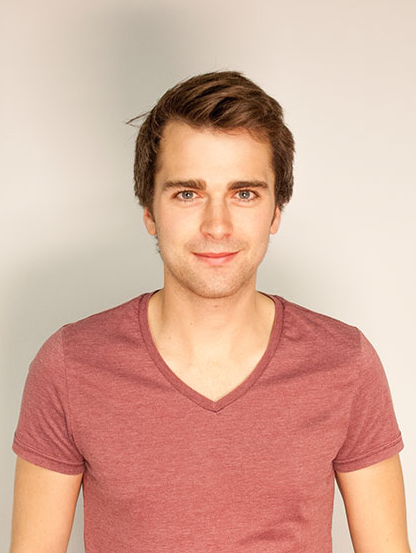
\includegraphics[width=0.8\textwidth]{portraitme.png} 
  \section{about}
  	born 10th January 1989
  	Gütersloh Germany
  	~
   	Am Lokdepot 3
    10965 Berlin
    Germany
    ~
    \href{mailto:mail@alexcmueller.de}{mail@alexcmueller.de}
    \href{http://alexcmueller.de}{http://alexcmueller.de}
    0176-34557235
  \section{languages}
    native German
    fluent English
    intermediate Spanish
  \section{programming}
    Python 3
    (Flask, Celery, Airflow)
    Java, Scala
    (Play Framework, Java 8)
    JavaScript
    (Node.js, React)
    NoSQL
    (Cassandra, Redis)
    SQL
    (Postgres, Vertica)
    \section{data analysis}
   	Python (scipy, numpy, sklearn, pandas, xgboost,jupyter)
   	Spark
   	Weka
   	Stanford Core NLP
\end{aside}
\section{Education}

\begin{entrylist}
  \eduentrythesis
    {2012 - 2015}
    {M.Sc. in Business Informatics}
    {University of Mannheim, ITESM Guadalajara(Mexico)}
    {Specialization in Data and Web science, exchange Semester in Mexico}
    {Thesis Topic:}
    {GPA (US) : 3.9, ECTS: A}
  \eduentry
    {2009 – 2012}
    {B.Sc Business Information Technology}
    {DHBW Mannheim in cooperation with SAP SE}
    {Specialization in Software Engineering}
    {GPA (US): 3.6, ECTS: A}
  \entry
    {until 2008}
    {University Entrance Qualification (Abitur)}
    {priv. Gymnasium Marienschule Lippstadt}
    {GPA (US): 3.4}
\end{entrylist}

\section{Experience}

\begin{entrylist}
  \entry
    {since 10 2016 }
    {Minodes GmbH, Berlin, Germany}
    {Lead Data Scientist}
    {Stuff}
   \entry
    {06 2015- 09 2016 }
    {Minodes GmbH, Berlin, Germany}
    {Data Engineer}
    {Data Engineer developing the Big Data Processing Pipeline enabling the WIFI-based Store Analytics, Introducing Apache Cassandra and Airflow during this time}
  \entry
    {09 - 10 2014}
    {Burda Bootcamp, München, Germany}
    {Developer}
    {Participant in a rapid prototyping lab (\href{http://burdabootcamp.de}{burdabootcamp.de})}
  \entry
    {02 - 08 2014}
    {SAP SE, Walldorf, Germany}
    {Data Science Student}
    {SAP HANA predictive maintenance development}
  \entry
    {2009 - 2012}
    {SAP SE, Walldorf \&  Darmstadt, Germany; Montreal, Canada}
    {Junior Software Developer}
    { Worked for different departments during the SAP Study program including SAP Research, CRM Consulting}
\end{entrylist}


\section{Theses, Publications and Patents}
\begin{entrylist}
	\entry
	 {2015}
    {Masterthesis}
    {University of Mannheim}
    {Towards An unsupervised Ontology Matching System using Outlier Analysis}
	\eduentry
	 {2013}
    {Publication}
    {University of Mannheim}
    {Binnig, Carsten; Salama,Abdallah; Mueller, Alexander C.}
    {XDB: a novel database architecture for data analytics as a service}
	\eduentry
	 {2012}
    {Patent}
    {SAP SE}
    {Doehring, Markus; Drittler, Bernhard; Kieselbach, Oliver; Mueller, Alexander Christian; Zimmerman, Birgit}
	{US20140058789 A1: Process model generation and weak-spot analysis from plain event logs}
	\entry
	 {2012}
    {Bachelorthesis}
    {DHBW Mannheim}
    {Design \& Implementation of a Process Mining Application for the Analysis of Weakspots in Business Processes based on In-Memory Database Technology }
\end{entrylist}


%\section{patents and publications}

%\printbibsection{misc}{other publications}
%\printbibsection{report}{research reports}

\end{document}
